\chapter{Fastype - Gamification of \ac{ned}}
\label{chap:gamechapter}
%Intro to the chapter
In the previous chapter we presented the named entity disambiguation framework which has been implemented as the initial part of the work conducted for this research study. The results after conducting a user study by using a plain interface which we called the AnnotateMe Interface indicate that non-expert users are able to perform qualitative annotations with the help of short contextual clues and an intuitive user interface. However, results also indicated seldom levels of frustration during the experiment in addition to a slight percentage feeling indifferent/neutral towards being engaged or positively motivated in performing the task. For the long-term run, we assume that the plain interface lacks elements of engagement and does not have any associated intrinsic motivation that will bring users back to perform annotations. We hypothesize that by gamifying the system appropriately, it will be possible to increase user engagement with the annotation task and thus increase intrinsic motivation for participation.\if If we manage to intrinsically motivate the users with the game design elements integrated in the annotation task than we are able to claim that it is possible to retain users for a long period of time which makes it possible to generate large-scale annotation corpora.\fi In this chapter we provide an outline of related gamified systems in the field of semantic web and natural language processing (\ac{nlp}) and background information on specific game design and theoretical models on which we base or work. The chapter proceeds by explaining the methodology used from the game implementation, preparation for the second user study and the metrics and assessment techniques used to analyze the data and report on the results. 

\section{Background}
\label{game:background}
%Pontsification - not enough
Gamification is not about taking an already existing system and decorating it with points, levels and leaderboards. This methodology of gamifying a system is referred to as "Pontsification" where the game design exclusively relies on points, badges and leaderboards \cite{47}. Zichermann et al \cite{48} argues that the technique of "Pointsification" comes as a result of lacking creativity and represents a poor approach to gamification. In order to create a gamified system that truly engages users and affects their needs for satisfaction, a game designer should put more work and effort than just throwing points, badges and leaderboards into the system hoping for users to feel engaged. 

The \ac{sdt} and its sub-theory \ac{cet} have been explained in Section \ref{thb:gamedesign} and serve as the foundations on which we base our gamification model and aim to reach the goal of positively affecting users needs for satisfaction, which (accrding to \ac{sdt} and \ac{cet}) results in increased intrinsic motivation. Before we proceed with state-of-the-art gameified systems, it is important to understand some key concepts that compose a well designed game. In gamification, the most frequently used framework is the MDA Framework \cite{47}. It is one of the most leveraged frameworks of game design and it is an abbreviation of the terms: Mechanics, Dynamics and Aesthetics.
% MDA framework
\begin{itemize}
    \item \textbf{Mechanics} compose the functioning of the game. Mechanics allow a designer to have complete control over the levels of the game, giving the ability to guide the players' actions
    \item \textbf{Dynamics} are the interactions of a player with the game mechanics. They determine the action of the player in response to the mechanics of the system
    \item \textbf{Aesthetics} of the game are the elements that define how the player is feeling during his/her interaction with the game
\end{itemize}
 
By carefully studying and exploring these models and frameworks when working on the game design, it will be genuinely possible to transform a system from being monotone and tedious to something that is interactive and fun to do. 

% Stats on game play 
A well designed game or gamified system can be used to gather large-scale amount of data and information. This data can potentially open doors to improving advanced systems such as search engines or helping scientific researchers find solutions to complex protein structures by using the computing power of the people (See Foldit \cite{53}). Entertainment Software Association did a survey to find out what are the characteristics of an average gamer and how much time gamers spent playing video games, and the following statistics were reported \cite{49}:
\begin{itemize}
    \item An approximation of 5 million Americans will spend 40 or more hours a week playing games, which is the equivalent of a full time job
    \item 60\% of Americans are gamers
    \item During 2013 the gaming industry was worth 22 billion dollars, with 16 billion spent on game content only 
    \item Females account for 50\% of gameplay and purchases
    \item The average gamer is 36 years old
\end{itemize}


\newpage
\begin{figure}[]
  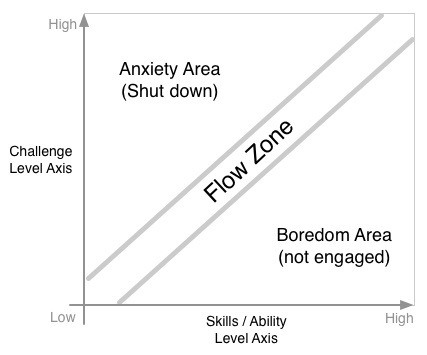
\includegraphics[width=.8\linewidth]{figures/experiment2/flowzone.png}
  \caption{The flow zone of a gameplay \cite{49}}
  \label{fig:flowzone}
\end{figure}
%Flow zone
A very important aspect in game design is the ability of maintaining the so called "Flow Zone" during the gameplay. The success of a game is achieved if the player is constantly kept within the flow-zone which is placed between anxiety and boredom \cite{49}. As illustrated in Figure \ref{fig:flowzone}, achieving flow or being in the "flow-zone" indicates the players' state of not being too overwhelmed with challenges but also avoiding the state of being bored because the game continues to offer easy challenges to the player. Zichermann et al. \cite{48} argues that a game designer must create a careful interplay of the system with the player by relentlessly testing their interactions until the point in which the player is between anxiety and boredom. This rule is applied from the first interaction of the player with the system which brings us to another quite important point in game design: Onboarding. 

%importance of onboarding 
According to Zichermann et al. \cite{48}, statistics from the casual games market show that the first minutes a player interacts with the game are the most important. This is because during the first minutes the player makes a decision whether he/she likes the game and will continue to play or not. Therefore, onboarding plays a crucial role to the overall success of the game. Onboarding is defined by Zichermann as the act of bringing novice players into the system. The responsibility of this part of the game is to carefully reveal the complexity of the system to the player without overwhelming him with too much information. In short, the goal of onboarding is to train and engage players but not overwhelm them.

%importance of challegne and other aspects (the bulletlist on the last th.b. page in the notebook about gamification).
Finally, some aspects which contribute to the idea of keeping the player engaged and motivated during gameplay need to be pointed out before we proceed with the next sections. According to Siemens et al. \cite{49}, a player expects the following elements from the game:
\begin{itemize}
    \item Focused goals
    \item Challenging tasks
    \item Clear and compelling standards
    \item Protection from failure
    \item Affirmation
    \item Novelty
    \item Freedom of choice
    \item Authenticity
    \item Affiliation with others
\end{itemize}
For our Fastype Game we have tried to employ most of these important aspects of game design in order to achieve high levels of engagement and intrinsically motivate players to interact with the game without any other form of incentive except the incentive of being entertained.
\section{Related Work}
\label{game:relate-work}
The emergence of platforms which contribute to the concept of having a group of individuals commit to creating a collective solution that is far more powerful and robust than individual ones has drawn the curiosity of many industries during the recent years. This concept is referred to as Collaborative Resource Creation (\ac{crc}) and is being utilized by systems that inherently want to use the creative and powerful nature of human thinking as a source of solving different computationally complex problems. Wikipedia can be considered as the best known example of collaborative resource creation. Furthermore, Open Mind Common Sense (\ac{omcs}) movement demonstrated that Web collaboration can be used as a tool to create \ac{ai} resource. Games can also be considered as \ac{crc} system. \cite{44, 43}

Wikipedia and \ac{omcs}, as non-gamified systems, rely on peoples' altruism and interest on science in order to commit to contributing. Whereas games provide the feeling of being entertained, and as a result the solely rely on user intrinsic motivations. Von Ahn et al. \cite{vonahn} argues that the desire to be entertained is a much more powerful incentive than any other incentive technique. It has been estimated that more than 9 million person-hours are spent by people playing games on the WEB. Dedicating a small amount of those playing hours to contribute to the solution of complex computational problems will result in tremendous benefits. This is the reason why Games With A Purpose (\ac{gwap}) are being frequently used in many domains such as \ac{nlp} and Semantic Web. Gamifying a system for the purpose of solving or facilitating computationally complex problems can be unquestionably powerful when doing it right. An excellent successful example of such a system is Foldit \cite{53}. 

Games are also used in education, generally as serious games and as digital game-based learning. In this field, gamification is defined as the use of game-based mechanics, aesthetics and game thinking to engage people, motivate action, promote learning and solve problems \cite{47}. Seaborn et al. \cite{47} argues that gamification has been used as a means of collaborative resource creation by numerous studies which take advantage of the alleged motivational benefits that game design can provide. However, almost all of these attempts of \ac{gwap} lack empirical research and standard of practice for design and implementation \cite{47}. In our work, we have attempted to analyze and understand empirical theories such as \ac{sdt} and \ac{cet} which guided the implementation of a \ac{gwap} for named entity disambiguation which resulted in a collaborative resource creation system generating training data for supervised \ac{wsd} and \ac{ned} algorithms respectively. 

Seaborn et al. \cite{47} also reported statistics on the usage of gamificaion across domains ranging from sustainability to health and wellness to education. The findings reported by the study indicate that the fields in which gamification has been mostly applied are Education (35\%), health and wellness (13\%), online communities and social works (13\%), crowdsourcing (13\%) and sustainability (10\%). They also report that a large majority of applied gamification research did not mention or address any theoretical foundations \cite{47}.

Gamification has been used as a mechanism to solve various \ac{nlp} and semantic web problems. Kaboom \cite{41} is a gamified \ac{wsd} system that can be classified as a 2D video game in the style of Fruit Ninja game. In this game, players are asked to destroy pictures that are not related to a specific term or concept shown to them beforehand. This approach aims to disambiguate word senses by using pictures as sense descriptors. The pictures that are kept at the end of a game round are considered to be related senses for the ambiguous word. Senses for each ambiguous word in the game were collected manually by expert annotators. Unlike them, we use our implemented microservice framework for generating game data instead of manually creating them, which gives us a headstart in focusing more on the game design aspect. Similar to our findings, Jurgens et al. \cite{41} also reported that game-based annotation systems reduce the cost of producing equivalent resources via crowdsourcing at least by 73\% while providing similar quality of annotations. Using Kaboom \cite{41}, they also reached a 16.3\% improvement in accuracy over state-of-art \ac{wsd}.

Phrase Detective \cite{44} is another gamified system that was developed to annotate corpora for anaphora resolution. Anaphora resolution is a semantic task used for recognizing that a pronoun like "it" and the definite nominal "the town" refers to some entity as a proper name \cite{44}. They argue that a successful \ac{gwap} should make use of all available incentives, namely, personal, social and financial. The game interface should be easy to use, intuitive to learn and designed to engage ones intended player demographic. Furthermore, they emphasize validation as a strong and effective method for quality control. By collecting multiple judgments for each expression, the gamified system can provide quality control and collect useful linguistic data. We employed some of the proposed methods by Phrase Detective as they proved to be appropriate for the design of our game, Fastype. 

To help with the creation of named entities, Green et al. \cite{50} developed the \textit{Entity Discovery} game where players are asked to annotate sentences by marking all named entities found in it. The game is played in pairs and when real players are not online to be paired with, a BOT is used instead. In order to validate the recognized entities by the first game, they developed a second game called \textit{Name that Entity}. The second game was designed as a multiple choice game were the paired players had to choose the type of the recognized entity. The game accepts a specific type for the recognized entity only if the paired players agree upon the type. \cite{50} 
In contrast, we automated the entity recognition task using our framework and for the validation task we use multiple judgments and rely on agreement levels between players which proved to be very effective and assured high quality of annotations. 

Several research studies investigated individual game elements and their impact on intrinsic motivation and performance \cite{43,45,46}. Badges, leaderboards and performance graphs, as reported by Sailer et al. \cite{45}, positively affected competence and need satisfaction. The same game elements also seemed to contribute to an increase in perceived meaningfulness as it is known that these game elements can create meaning at the game level \cite{45}. Unsurprisingly, Mekler et al. \cite{46} found that pontsification (points, levels and laderboads) functioned as extrinsic incentives effective for promoting performance quantity. They used an image annotation game to determine the effect of these three most commonly employed game elements on needs satisfaction, intrinsic motivation and performance. Using a two-fold experimental study, the game element group performed better in terms of annotation quantity, whereas the quality remained the same. Against their expectations, the different conditions (groups) did not differ in terms of intrinsic motivation or competence as a factor that impacts needs satisfaction. Possible factors that contributed to this outcome is that the game did not provide enough challenge to the players, the feedback was insufficient in determining player performance and the game lacks visual and aural presentation of game elements and feedback to the player. We try to overcome these obstacles by designing a game that keeps the user constantly engaged by increasing challenge as the player progresses, provide visually appealing feedback, empowered social elements, encouraging self-empowering through performance graphs etc. 
\section{Game Design}
\label{game:design}
Games With A Purpose (\ac{gwap}) are implemented in many fields and come in various forms. With regards to their overall game design, they tend to be graphically rich, provide simple interactions and give the player an experience of progression by scoring points, leveling players up and recognizing their effort. Additionally, the design of the game should reinforce quality measures and control the behaviour of players. Encouraging players to concentrate on the task and discourage them from malicious behaviour is crucial for quality control \cite{42}. The goal of our research study was to develop a \ac{gwap} that would serve as a tool for validating the named entity disambiguation task. The validating process should be performed at the highest quality level possible and still maintain player engagement by positively affecting their intrinsic motivation: experiencing feelings of competence, autonomy and relatedness while playing. The following subsection explore the different game elements and the corresponding game design principles used in Fastype that make this game enjoyable, fun to play and motivate players to come back and play. This results in generating large-scale annotation data for our named entity disambiguation task without players noticing what the underlying purpose of the game is.

\subsection{Onboarding}
%Onboarding 
The first impression you get when meeting somebody for the first time is usually a strong indicator that determines whether you will like the company of this new person or not. Similarly, the first impression or the first minutes of interacting with a game are the most important because a player will make a decision whether he or she will continue exploring the game. According to Zichermann et al. \cite{48}, the onboarding process is critical to a successful game. A good onboarding process leaves no other options to the player but to win. It is crucial that in this stage the player will be offered with an action at which he will not be able to fail. After having completed the initial action/task, the player should be rewarded for successfully completing it. \cite{48, 43, 48}

During the implementation of Fastype, special attention was put in designing the onboarding phase as effective as possible. Fastype has been designed as a typing game where players have to type on their keyboard as fast as possible to reach high scores and improve their typing skills. Additionally, the game requires the user to focus and memorize what they type in their keyboard and also answer quiz-like questions to get additional points, reach new levels and complete various categories. All these concepts have to be carefully revealed to the player during the onboarding stage. According to Zichermann et al. \cite{48}, the onboarding process should accomplish the following things: 
\begin{itemize}
    \item Slowly reveal the complexity of the system
    \item Positively reinforce players
    \item Avoid any action that leads to failure
    \item The game should learn something about players in order to personalize the game if necessary 
    \item All the points mentioned above have to be done within the first few minutes of the player interacting with our game
\end{itemize}

Except the points listed above, we also wanted the onboarding process to be slightly intriguing and mysterious in order to tease the player's curiosity. When entering the game site, the players are presented with a screen which requires them to know a \textit{ game secret} (See Figure \ref{fig:game-startscreen}). Having a secret comination to enter the game might potentially affect feelings of relatedness as the player will experience feelings of being part of a secret game club which allows entrance only to players who are aware of the game secret. However, the game provides a way of discovering the game secret. The only way of acquiring it and being granted with access to the game is by following a trial procedure. This trial procedure represents the onboarding process for our game. 

\begin{figure}[h]
  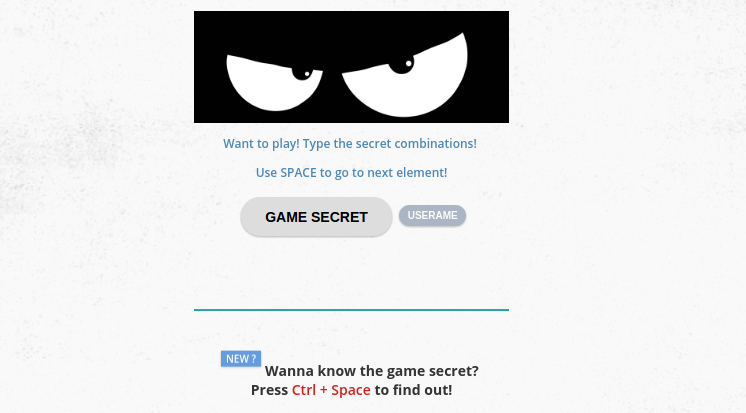
\includegraphics[width=\linewidth]{figures/experiment2/startscreen-game.png}
  \caption{The game start screen presented to player when entering the game for the first time}
  \label{fig:game-startscreen}
\end{figure}


The onboarding process starts by asking players to type the words that appear in the screen as small boxes. Points are awarded to the player regardless of their typing speed (rewarding and recognizing the players' effort). After the player is familiarized with the way the game works (typing fast while paying attention to the words that appear in the screen), the game continues by introducing a new challenge: a puzzle combined with typing skills. The puzzle consists of several hidden characters that the player has to reveal by typing the words appearing in the screen. The faster the typing the faster the revealing of characters. After the player has revealed all the characters on the puzzle, he is presented with a quiz where the \textit{question} is the revealed word (i.e. the named entity) and the options are the candidate entities extracted from \ac{kb}. Contextual clues are provided on top of the screen as sticky notes which help the player to make a correct decision. The quiz is a \textit{masked} version of the named entity disambiguation process used in the first experiment. The player proceeds by selecting a candidate option which is rewarded with 10 game points. Please note that if the player selects the wrong option, the system will not proceed until the right option is selected. As a reward for choosing the correct answer, the player finally reaches the end of the trial process where the game secret is finally revealed. Additionally, the player has to register himself with authentication credentials which together with the game secret are used as a secret combination for granting access to the game. Figures \ref{fig:onboarding}(a) to  \ref{fig:onboarding}(f) illustrate the complete onboarding process of Fastype. 

\begin{figure}[]
  \centering
  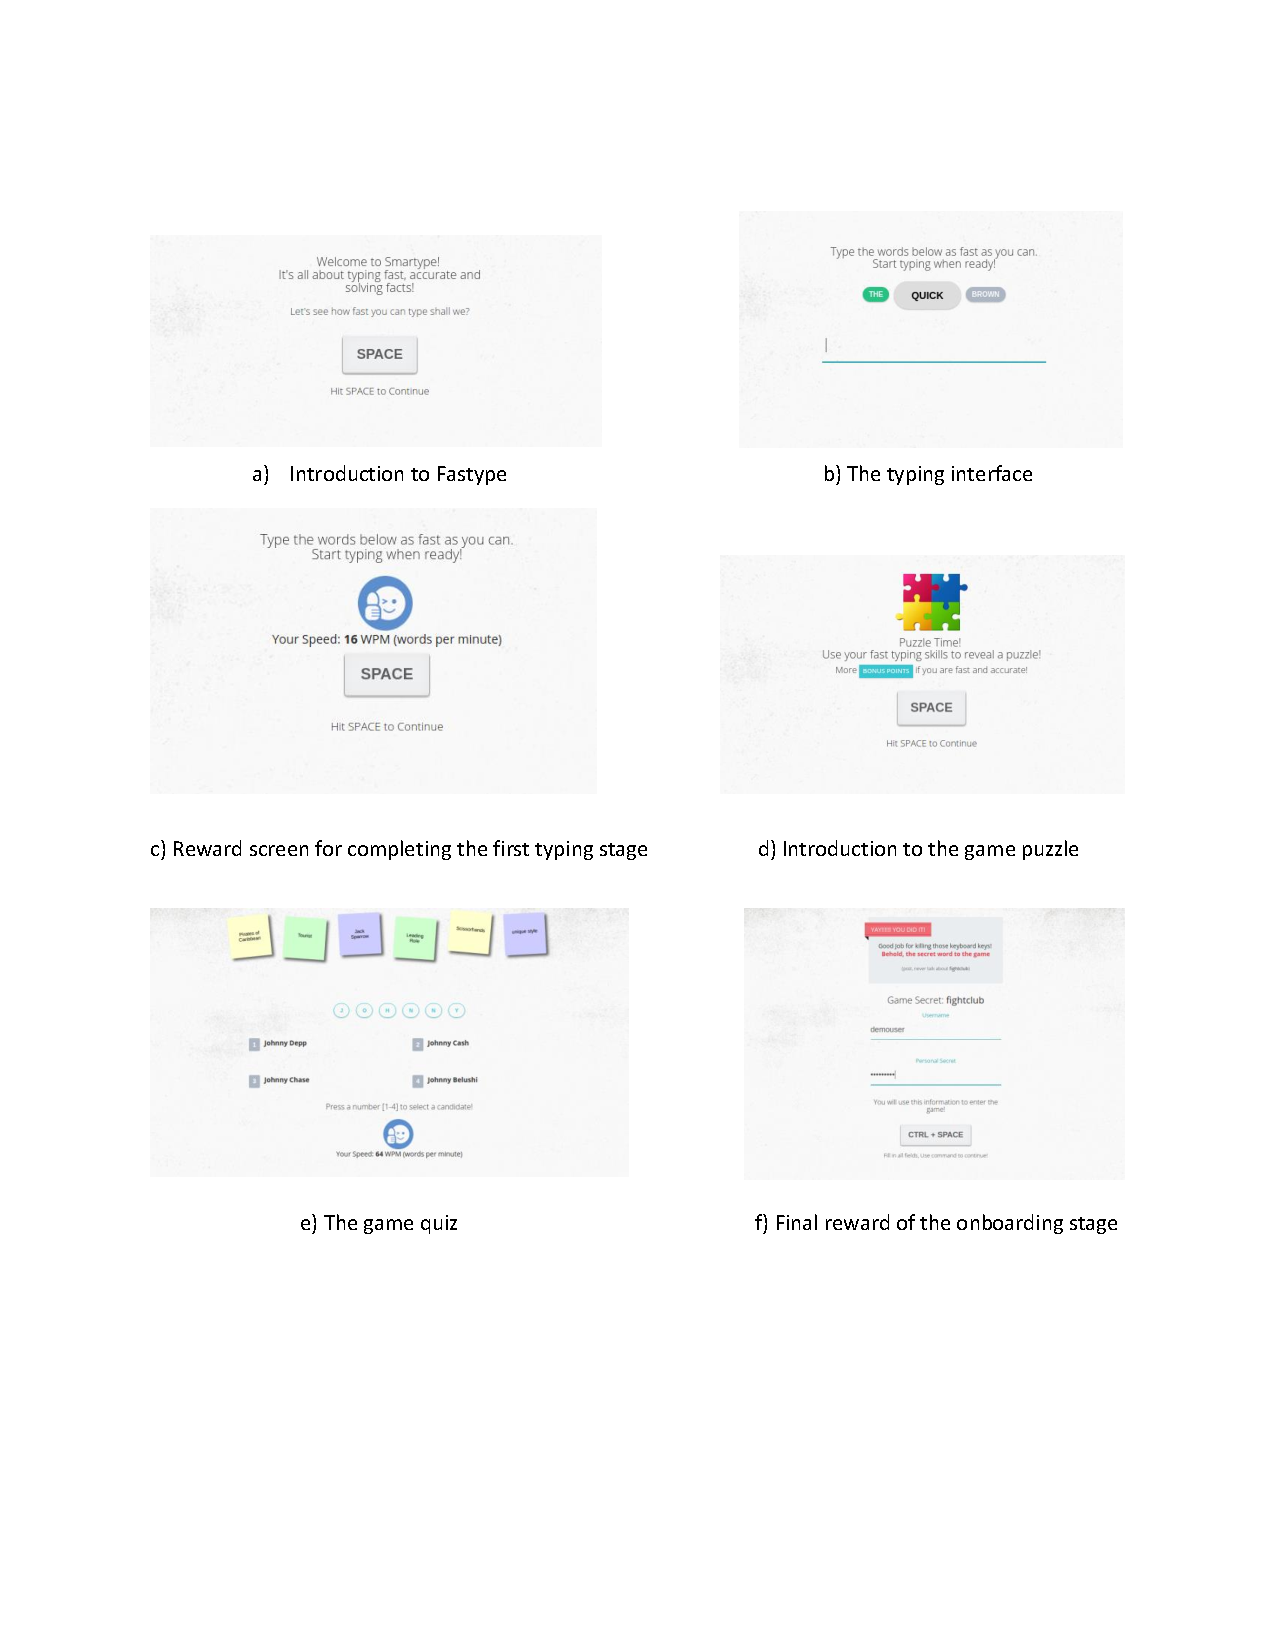
\includegraphics[page=1,width=\textwidth]{figures/experiment2/oboarding.pdf}
  \caption{The onboarding stage of Fastype}
  \label{fig:onboarding}
\end{figure}
\subsection{Task Design}
After exploring and analyzing many gamified systems and the effect of various game elements towards user engagement and motivation, Sailer et al. \cite{45} argues that gamification is not effective per se, but specific game design elements have specific psychological effects. Thus, it is important that gamification is not done just by incorporating a scoring system with some levels to advance and a leaderboard to see your progress. It takes more than that to design a game that attracts and retains a player base. 

Chamberlain et al. \cite{43} emphasizes that it is the design of the individual tasks in a gameplay that determine how successful the player can contribute data whilst playing. Furthermore, Sailer et al. \cite{45} communicates the importance of game elements being recognized by the player in the gamified environment. Delivering the treatment to the player or to a participant in the game is not enough unless the designer of the game makes sure that the treatment is also received by them. Failing to design treatments or game elements that are genuinely recognized by the players, results in loss of statistical power and risk to underestimate their effectiveness \cite{45}. In order to adhere to the aforementioned design constraints, significant work effort was placed in designing a task that contributes to generating annotation data of good quality. 


A game-round starts by the player selecting a specific category to play or letting the game choose a category in a random fashion for the player. Everything in the game is designed in a way that the player only has to use the keyboard for completing almost every action. The player is then presented with the typing screen where a combination of hidden characters have to be revealed by typing as fast as possible. Figure \ref{fig:game-typingscreen} illustrates the typing screen. A speed radar is placed right underneath the typing text box which displays the current speed of typing measured as the amount of words typed per minute while the player is revealing the hidden characters. This element can be considered a strong motivator to keep the player focused on typing fast. After having revealed the word, the upcoming challenges/questions all revolve around the text that has been typed during the typing phase. The players are already familiar with this concept since a similar task was already performed during the onboarding phase. Bonus questions are immediately presented to the user after completing the revealing stage (we talk more about the importance of bonus questions towards the overall design in a later subsection). The content of the bonus questions is created by using the text that was typed in the previous stage. Similarly, the most important part of the game that contributes to the original task of disambiguating entities is the quiz stage of the game. The quiz interface provides contextual clues extracted from our original framework and lists all the potentially candidates (quiz options) from which the player has to choose. 

\begin{figure}[]
  \centering
  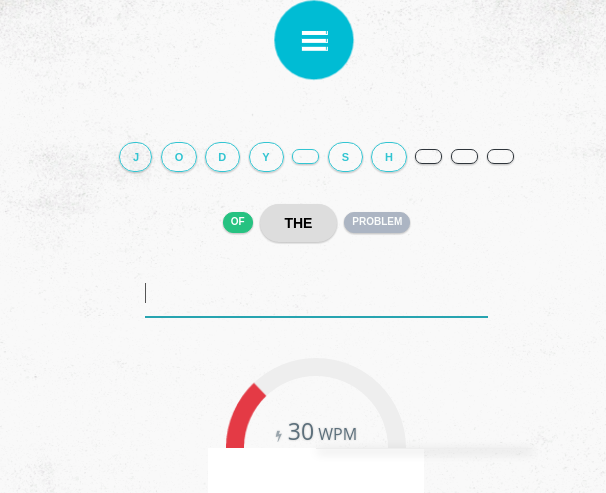
\includegraphics[width=.6\linewidth]{figures/experiment2/gameplay1.png}
  \caption{The typing screen and the speedometer calculating the typing speed of the player}
  \label{fig:game-typingscreen}
\end{figure}

We strongly emphasize the fact that all the game elements presented so far are focused and contribute to the ultimate goal, which is annotating the entity with the right candidate. The text which the player types during the typing stage, the content of the bonus questions and the contextual clues all represent carefully carved information that contribute in helping the player choose the right candidate. We make sure that the typing text\footnote{During the fast-typing stage, players are presented with different words that appear on the screen one after another. These words are part of a complete paragraph that is taken from the document where the target entity is part of.} as a game element is recognized and takes the attention of the player because if players are able to remember the text they typed, they can get points from correctly answering the bonus questions and also be confident on the candidate option they select. An example of a bonus question is presented in Figure \ref{fig:game-bonusqeustion} while the quiz interface of the game is illustrated in Figure \ref{fig:game-quiz}. 

\begin{figure}[]
    \centering
    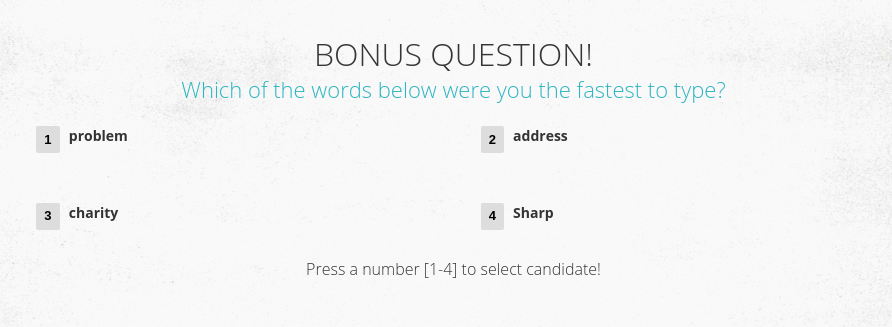
\includegraphics[width=.8\linewidth]{figures/experiment2/bonusquestion.png}
    \caption{An example of a bonus question}
    \label{fig:game-bonusqeustion}
\end{figure}

\begin{figure}[]
    \centering
    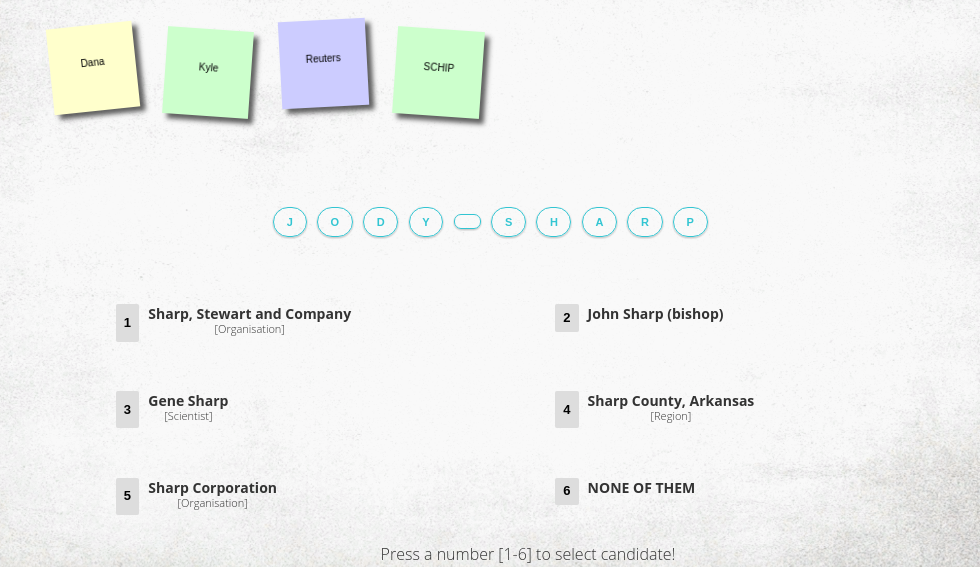
\includegraphics[width=.6\linewidth]{figures/experiment2/game-quiz.png}
    \caption{Interface of the game quiz - a gamified version for the named entity disambiguation task}
    \label{fig:game-quiz}
\end{figure}

%Skillset required/improved in the game
Schell \cite{51} (page 214) emphasizes the importance of the skill and chance mechanisms in games. A good game should balance between skill and chance during the gameplay. We believe that we have reached a satisfactory balance between these two factors by equalizing the factor of chance and skill required. The factor of luck is represented by bonus questions which are extracted from the typing text and are genuinely hard to answer since a memorization of everything typed is required. On the other hand, the factor of skills is represented by the quiz element of the gameplay. Correctly answering the quiz requires certain skill-sets from the player in order to maximize their profit point-wise. Except requiring skills from the players, the game should also contribute in allowing the players to master and perfection these skills. In general, by playing Fastype, a player will improve the following skills:

\begin{itemize}
    \item Typing skills
    \item Concentration in time pressure 
    \item Memory training and pattern recognition
    \item Knowledge in different categories (politics, music, entertainment, health etc)
\end{itemize}

Improving these skills is one of the goals that players will attempt to achieve. After having observed the players during their gamplay when conducting the second experiment we are aware that the goals of the game are concrete, achievable and rewarding at the same time. Having all these three elements characterizing the goals of the game is crucial to keeping players engaged and motivated \cite{51}. 

Reviewed literature suggests a number of criteria for evaluating enjoyment during gameplay. Some of the criteria which apply to task design and which also relate with SDT in terms of their importance towards increasing intrinsic motivation include: Feedback and Immersion \cite{41}. Constant feedback is given to the player for every performed action when interacting with Fastype. Immersion in our case refers to a short and arcade style of the gameplay which make the player experience a deep and yet effortless involvement in the game \cite{41}. A game round in Fastype lasts 4-5 minutes on average with the player being exposed to different challenging tasks. This results in an effortless and deep involvement in the game for a short period of time. Additionally, the game elements and the feedback provided during the gameplay have been enriched with sounds, visuals and animations which according to Mekler et al. \cite{46} can positively affect competence, needs satisfaction and subsequently increase intrinsic motivation.

%performance graphs, levels, leaderboards, points 
Game elements such as performance graphs, levels, points and leaderboards are provided in the game in order to give the players the feeling of progression and advancement. With these game elements we also reinforce the competitive nature of players to compete with others but also work hard on breaking their personal best scores. This results in encouraging players to get better each time they enter the game (mastery of skills). Figure \ref{fig:game-profile} illustrates the profile of the player where a performance history of the typing speed is provided in addition to level information, challenge status and betting ratio (a balance between the bets lost and won).

\begin{figure}[]
    \centering
    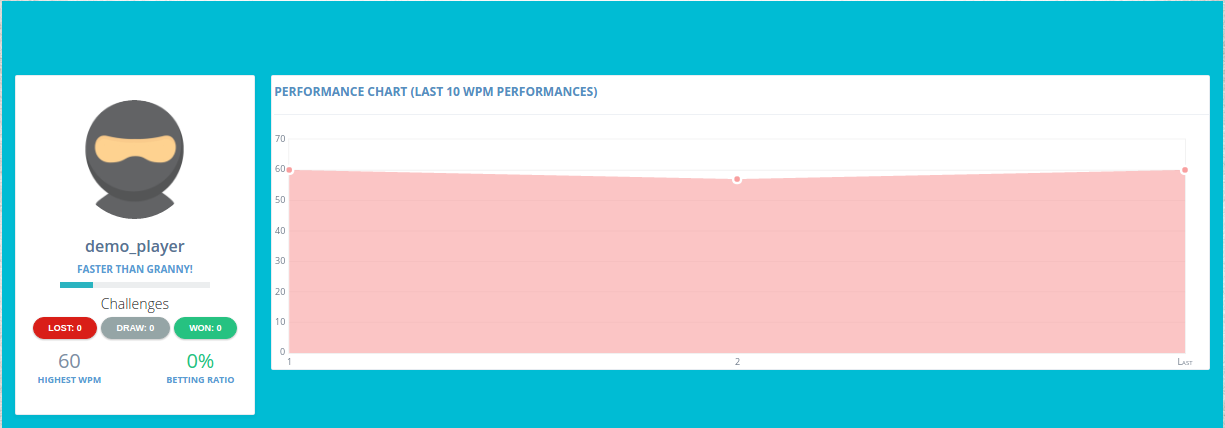
\includegraphics[width=\linewidth]{figures/experiment2/profile.png}
    \caption{Player profile screen}
    \label{fig:game-profile}
\end{figure}

The final element that requires our attention is the concept of game-flow. It was explained in the background section of this chapter that game-flow is the concept of keeping the player constantly engaged while not overwhelming him with problems that are too complex to overcome or too easy that the player gets bored quickly. Our idea of keeping the complexity of the game in the same level as the player's progression and skill improvement in the game is by increasing the total number of words that players have to type within a game-round. The complexity is controlled by the level mechanism of the game. When players progress and reach new levels, they are faced with longer and more complex paragraphs to type. However, one can argue that this is not the best and most optimal way of maintaining game complexity and player's flow zone. Being limited in the amount of resources available to be spent in designing and implementing all the game elements, the proposed idea of defining and maintaining game complexity was the only achievable concept within these constraints. However, ideas to improve the existing design of game complexity will be addressed in the discussion section and as such will be accounted for future work. 

\subsection{Freedom of choice}
%Autonomy - Freedom of choice - categories 
%training phase
During the first experiment where the non-gamified interface was used to perform annotations, many participants addressed the fact of not having control over the genre of the entities presented to them. Since the selection of the entities to be resolved was done in a random fashion, one of the participants was constantly getting entities that fell into the Arts category. As a consequence, the participant was feeling very insecure during the task because of being unfamiliar with most of the concepts being presented to him. We would like to stress out the importance of freedom of choice in this aspect. Being able to freely decide what category to play in, is an important factor for reinforcing autonomy and competence. As a result, the game gives the player the freedom of choice by providing several game categories to choose from. For players who like the aspect of surprise and chance, the game can make a random choice for the player if instructed to do so. 

Furthermore, the game provides a training phase for players who feel unprepared to take the actual task where the performance is recorded. According to Chamberlain et al. \cite{43} GWAP usually begin with a training phase so that players are able to practice their skills and also show that they have understood the instructions before they do the real task. However, in our case the onboarding stage takes care of explaining the complexity and instructions for performing actions in the game while the training phase allows the user to practice their typing skills. The training phase was also designed for the purpose of getting familiar with a new keyboard since the participants played the game from the experimenters laptop and therefore it was necessary to have a training phase. The game acknowledges the player for the existence of a training possibility in the game by pushing notification on the screen.
\subsection{Game challenges}
%Challenges 
%Punishmet
Von Ahn in his pioneering work \cite{vonahn} focuses on one type of incentive to motivate players: enjoyment. He emphasized that the main mechanism to make players enjoy a GWAP is by providing them with a challenge. Usually in many gamified systems, challenges are achieved through mechanisms such as requiring a timed response, keeping scores which ensure competition among players, having players with similar level of skill compete against each other and so on. \cite{44} 

The design of Fastype strongly reinforces the competitive nature of players by providing challenges which allow players to compete with each other. During each game round, the system keeps track of the player's typing speed, and shows potential challenges based on their WPM (Words Per Minute) accordingly. To assure fair play, the system makes sure that the player is presented with challengers that have roughly the same level of skill. The challenge screen is presented to the player after she has completed the quiz. Figure \ref{fig:game-challenge-screen} shows the exact challenge screen which is used by players to send challenge requests to other players in the game. As seen in the figure, players can choose a number of points between 1 and 10 to challenge the other players. These points represent the reward or punishment mechanism of the challenge. To assure fair play of the game, players who are challenged will type the exact same words as the challengee, therefore an accurate measure of their skill is guaranteed. Finally, having a challenging game where each challenge matches the players skill level contributes to the feeling of enjoyment during gameplay \cite{43}.

\begin{figure}[]
    \centering
    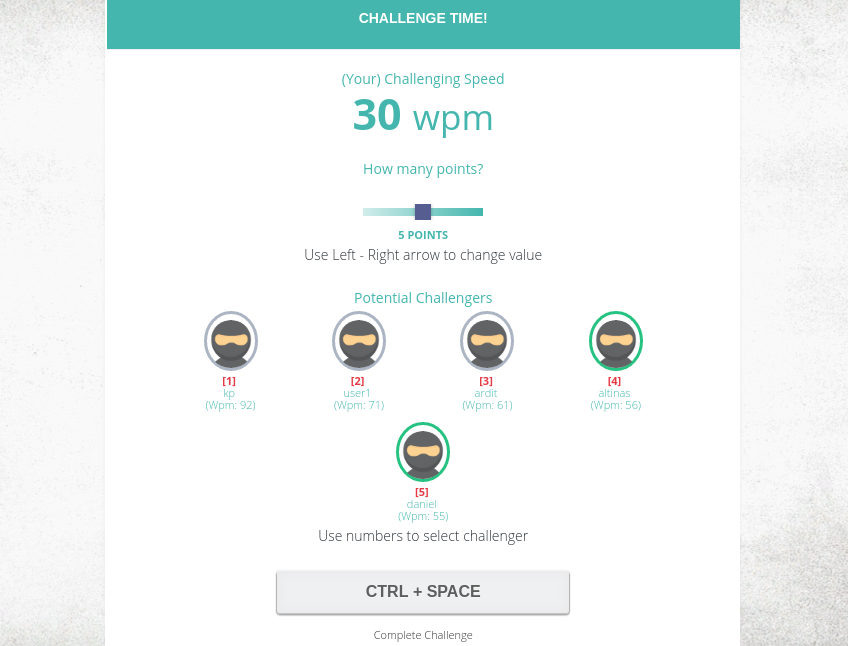
\includegraphics[width=.8\linewidth]{figures/experiment2/challenge-time.png}
    \caption{Fastype Challenge Screen}
    \label{fig:game-challenge-screen}
\end{figure}

An additional note that requires attention is the mechanism of punishment in a game. Schell \cite{51} (page 225) addresses the importance of punishment mechanisms in games and if balanced appropriately, they will give more meaning to everything in the game. Punishment mechanisms increase the value of certain game elements such as points. In Fastype, challenges and the betting mechanisms provide a way of punishment for players. In case of failure, their accumulated game points will be taken away, subsequently dragging the player down in lower levels in addition to increasing the failure percentage in their profile. Please note that the players have always the option of skipping challenges or bets on their answers. As a consequence of avoiding challenges and bets in the gameplay, the player will experience a slow progression and less dramatic gameplay as compared to other players who take risks by betting and challenging other players.
\subsection{Bonus Questions} 
%lens of chance
%the element of surprise, random nature (never know what to expect), have to rembmer all what was written and how it was written, a skill which is hard to master but interesting and misterious and with the help of chance it is sometimes easy achieved
The bonus questions represent the element of chance and surprise in our gameplay. The random nature of the bonus questions give the game a unique flavor of mystery and surprise since the player never knows what to expect from the bonus questions and therefore it encourages players to work on remembering what and how she was typing. Some bonus questions ask about the total number of words typed, the fastest word typed, the number of times a player failed to type a word correctly, the number of times a specific word occurred etc. The bonus question play an important role in the overall playfulness and feelings of enjoyment during gameplay. 
\subsection{Betting System - a measure for quality control}
Many of the existing gamified systems point out the importance of quality control in \ac{gwap}. Von Ahn et al. \cite{44} suggests two mechanisms for ensuring correctness of data: player testing \footnote{Player testing is evaluating the players output by occasionally matching it against gold standards or already annotated data} and repetition or redundancy of data. In our game design we have employed two mechanisms for ensuring that the quality of annotations performed through the game is maintained. 
The first assessment methodology is accumulating multiple individual answers for a specific entity before deciding whether that answer is correct or not. This corresponds to the redundancy of data for quality control suggested by \cite{44}. The second assessment methodology is using the betting system incorporated into the game. If we look at the betting element in the game from the eyes of a game designer, this element represents the lens of triangularity proposed by Schell \cite{51} (page 212). The lens of triangularity gives a player the choice to play safe for small rewards or take a risk and win big rewards. Triangularity gives an interesting and exciting flavour to our game. On the other hand, if we look at this game element from the eyes of a linguistic expert who demands from the game the generation of trustful and qualitative annotations, than this element represents a measure for assessing the confidence of a player towards the his choice of candidate. Figure \ref{fig:game-bet} illustrates the betting screen shown to the player immediately after having completed the quiz.

\begin{figure}[]
    \centering
    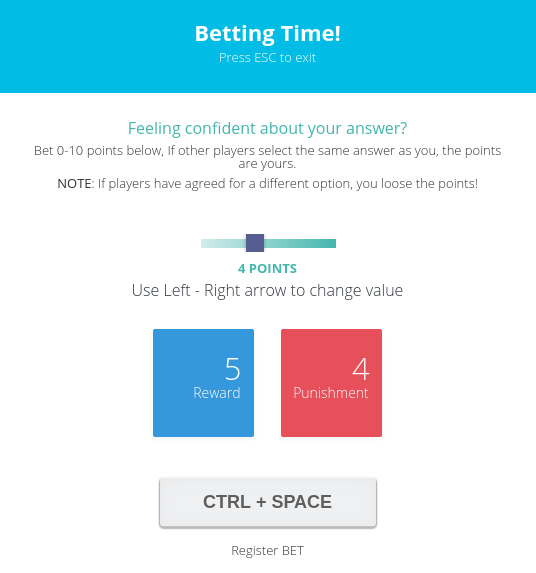
\includegraphics[width=.8\linewidth]{figures/experiment2/game-bet2.png}
    \caption{Betting Mechanism as a quality control and representative of triangularity for Fastype}
    \label{fig:game-bet}
\end{figure}

As we can see from Figure \ref{fig:game-bet}, the player has the choice of deciding the amount of points he wants to bet on the selected answer. The bigger the number of points used in the bet the higher the risk of loosing or wining them. Players are instructed to think if other players who might potentially encounter the same quiz will also choose the exact same answer as they did. In that case, if they are confident about the given answer, then the players are encouraged to place high bets rather than playing it safe. However, the choice remains completely in the hands of the player. Our betting mechanism works in the way that for one individual entity, when more than 4 unique judgments agree on the same candidate, than this entity is considered to be resolved. All the players whos' selected candidate is the same as the correct candidate (meaning their answer falls within the absolute majority) will be rewarded with the amount of points they bet for the particular entity. Similarly, all the players whos' answer was not the one selected by the majority are punished by subtracting the amount of points they bet from their overall accumulated points in the game. In terms of annotation quality, candidates with higher betting scores represent higher levels of confidence which means we can be sure that the selected candidate is undoubtedly the correct representative for the target entity.
\subsection{Social Interaction \& Engagement Loop}
%SHoutouts, challanging, desire to compete (being the first in the board) each other as relatedness factors - increasing social interaction - Relatedness is a factor that positively affects intrinsic motivation
Significant design and implementation effort was put in making the game as much socially interactive as possible. Among the three SDT elements which have direct impact in intrinsic motivation and needs satisfaction, social interaction contributes to the feeling of relatedness with others. The main social interaction mechanism implemented in the current version of the game are challenges. The desire to compete and overcome players in the leaderboard can be seen as an element that entails social interaction within the game. 

%engagement loop
The concept of engagement loop on the other hand is a fundamental aspect that needs to be clearly defined in order to maintain player motivation. A successful designed engagement loop always leaves something incomplete or pending in the game for players to come back and play. Game designer David Perry suggests that the key to addictive game design is by creating a game that keeps the player engaged by doing three things all at the time: exercising a skill, taking risks and working out a strategy \cite{15}. Zicherman et al. \cite{48} gives substantial importance to the social engagement loop and defines the following four key aspects to be considered by game designers when thinking about engagement loops: motivating emotion, player re-engagement, social call to action and visible progress/rewards. Table \ref{tab:engagement-loop} lists the game elements of Fastype that contribute to the different aspects of social engagement loop.

% Table generated by Excel2LaTeX from sheet 'Sheet1'
\begin{table}[htbp]
  \centering
  \caption{Game elements of Fastype that contribute to the social engagement loop}
    \begin{tabular}{|c|l|}
    \toprule
    \multicolumn{2}{|c|}{Social Engagement Loop} \\
    \midrule
    \multirow{Motivating Emotion} & Excercising fast typing \\
          & Competing with others \\
          & Learning new facts  \\
          & Improving Memory skills \\
    \midrule
    \multirow{Player Renegagement} & Levels \\
          & Challenges  \\
          & Increasing WPM  \\
          & Completing Categories \\
    \midrule
    \multirow{Social call to action} & \multirow{Challenges } \\
          &  \\
    \midrule
    \multirow{Visible progress} & Leaderboard \\
          & Points  \\
          & Levels  \\
          & Challenge Win/Lose Ratio \\
    \bottomrule
    \end{tabular}%
  \label{tab:engagement-loop}%
\end{table}%
\newpage
\section{Methodology}
\label{game:methodology}
% DESCRIBE THE METHODOLOGY USED TO ANSWER THE FOLLOWING RESEACH QUESTIONS

%---- What game mechanics can be employed in the entity resolution task so that high levels of engagement are achieved while still maintaining annotation quality?
The last proposed research question posed by this study is concerned in finding out what game mechanics and design principles are best fit for our research problem in order to positively affect intrinsic motivation and achieve high levels of engagement. We are also concerned to find out whether the implemented game contributes to qualitative annotations by non-experts so that we can harvest the potential of players with different levels of expertise in annotating, age group and academic background. To be able to answer our third research question and assess the usability and performance of our implemented game, we conducted another experimental user study with the same participants who participated in the first experiment. However, a different dataset was used for the second experiment. Choosing a different dataset was important since the participants were already familiar with the two datasets used in the first study. 

%Datasets 
%--Describe the stats of the dataset, nr of entities, types etc
MSNBC first introduced by \cite{24} is the dataset used for our second user study. It contains news-wire text from MSNBC news network. The dataset was created in 2007 and contains information and facts from that period. This fact was communicated and acknowledged by the participants on the second experiment in order to avoid reference errors such as linking the entity "USA President" with the candidate "Donald Trump" instead of "George W. Bush". The complete dataset contains 20 document in total, however, we used only 12 of them in order to reduce the total number of entities to deal with. Experimenting on a reduced version of the dataset instead of the complete version does not have any implications on our results. The reason we used a reduced version of the dataset is because our game relies on multiple judgments to disambiguate an entity (4 independent judgments to be precise). Therefore, having a small pool of entities to pick from would result in more entities being resolved during our time limited user experiment. The more entities resolved during the experiment the more confident the results of our analysis. In summary, we used the documents in the following categories from the MSNBC dataset for our second experiment: Entertainment, Health, Politics, Technology, Sports and World. The gold standard for MSNBC reported 251 named entities in total with an average of 20 named entities per document.   

%recruiting participants
%--Describe the experiment (setup, duration)
%-- we used the same participants as in the last experiment 
%-- not all showed up because of sickness or not being at the campus at the time of experiment
Similar to the first experiment, emails and social media were used as communication sources for recruiting participants for the second experiment. Initially, we aimed to recruit the same participants who took part in the first experiment, however, since some of the participants reported to be away or sick during the time of experiment, we sent invitations to others as well. As a result, 26 participants took part in the second experiment with 24 of them participating for the second time. 

The university campus was the environment where the second experiment was conducted. Participation was scheduled in different time-slots with a maximum duration of 40 minutes assigned for each round. Stretching the session duration to 40 minutes has been done for the only reason of giving temporal space for participants who wished to play longer if necessary. During the invitation process, it was made clear to the participants that the (mandatory) duration of the experiment would be approximately 20 to 25 minutes including the pre-questionnaire, gameplay and post-questionnaire. Similar to the first experiment, we used a consent form to communicate the purpose and the voluntary nature of the experiment. In order to assure consistency of data given by participants, a pre-questionnaire gathering demographic information was also used in the second experiment in addition to questions related to frequency of playing video games. We report on the demographic data of participants and their frequency of playing video games in section \ref{game:results} whereas the questions used in the pre-questionnaire are presented in Appendix \ref{appendix2:fastype}. 

% Assessment methodologies
The completion of the pre-questionnaire was followed with an immediate transition to the gameplay. In order to be consistent with the first experiment, players were asked to perform game rounds iteratively until the experimenter instructed them to stop. 15 minutes were dedicated for performing game rounds (annotations). However, the game includes an onboarding phase which introduces the player with the game and gradually reveals the complexity without overwhelming the player with too much information at once. Therefore, the time used by each participant to complete the onboarding phase is not recorded as part of the 15 minutes of total gameplay. The reason is that no annotation is performed during the onboarding phase of the game. After the 15 minutes of gameplay, participant were told to either finish playing or continue as they desire. This methodology was used in the first experiment as well and allows us to assess the participant's engagement with the game and its fun aspect. Finally, a post-questionnaire was used to assess player engagement, motivation, usability and enjoyability of the game. We report on the results of the post-questionnaire in section \ref{game:results} and list the questions used in this questionnaire in Appendix \ref{appendix2:fastype}.

Agreement level with the majority and comparison of game annotations with the gold standard are the methodologies used for determining the quality of annotations performed by players while playing Fastype. Besides the free-will annotation metric used in the first and second experiment for assessing the level of engagement of participants with each interface, we also employed Von Ahn and Debish \cite{44} assessment metrics for evaluating a GWAP. Von Ahn proposes two assessment metrics: \textit{throughput} which represents the speed at which a particular player is annotating, and \textit{average lifetime play} which represents a measure of enjoyability \cite{44}.


% ANOVA for comparison of game and interface, differences in number of observations, does not have any impact on results when working with small samples
Additionally, in order to report confident results, it was necessary to perform ANOVA analysis between the two conditions (AnnotateME and Fastype) for different factors such as: enjoyability, level of engagement and the likeliness of participants  to use each interface for an actual task outside the experiment. We perform one way ANOVA analysis for this purpose. For the sake of reproducability of results, it is important to note that the observations used to calculate ANOVA for the two conditions were not the same. The observations from the second experiment were slightly smaller than those from the first experiment. However, from a statistical point of view, small differences between conditions do not affect the final results when calculating one way ANOVA. Please note that ANOVA analysis were manually performed using Excel spreadsheets. Finally, to support our claims that the Fastype game was significantly more engaging and fun to play compared to the AnnotateMe interface, besides evaluating the interfaces using the aforementioned assessment metrics we sent a final assessment questionnaire to all participants who took part in both experiments. The questionnaire consisted of one question which asked about their preferred interface for performing the task of resolving named entities. This answers to the last questionnaire allow us to strengthen the claims that the game was significantly more attractive compared to the non-gamified interface. The content of the questionnaire is presented in Appendix \ref{appendix2:fastype}.  

% Likely sources of BIAS


%Hypothesis 
\paragraph{Hypothesis}
The second experiment was conducted in order to determine whether our proposed gamified system can intrinsically motivate users to perform a tedious and boring tasks such as named entity disambiguation. Another important aspect that needs to be emphasized is the quality of annotations. It is crucial for the design of the game to avoid having distracting elements that would intentionally or unintentionally degrade the quality of annotations. Keeping these important aspects in mind, we hypothesize that: 

\begin{itemize}
    \item H2.1: By employing game mechanics and design principles based on theoretical foundations, players will be intrinsically motivated to play the game
    \item H2.2: In case H2.1 is supported, we can further hypothesize that users who have used both interfaces to perform annotations will choose the game significantly more than the plain interface.
    \item H2.3: The quality of annotations performed by players will not be degraded even after implementing game elements that do not directly contribute to the annotation task.
\end{itemize}
\newpage
\section{Results}
\label{game:results}
This section reports on the results after conducting the second experiment and analyzing the effects of the different game elements towards user engagement with Fastype. We also report on the playfulness of the game, feelings of competence, autonomy and relatedness in addition to testing and comparing the quality of annotations with the first experiment. In overall, these analysis will guide the rest of this research study towards answering the last research question regarding gamification and the corresponding hypothesis.

\subsection{Participants}
%Pre questionnaires 
%difference compared to first experiment 
It was mentioned in the previous section that the recruitment of participants has been done in a consistent way with the first experiment. The participation resulted in having 27 participants in total which is 3 participants less than the first experiment. Those who did not show up for the second experiment were either not at the university campus during the whole week of experiment or were sick and could not show up. However, among those 27 participants 11.1\% (namely 3 out of 27) of them were partcicipating for the first time. This small group of participants that were not part of the first user study were not presented with questions that involved comparisons or assessment of AnnotateMe with Fastype.

The pre-questionnaire for the second experiment was designed for gathering information about players' demographic data in addition to information related to their gameplay frequency. The questions related to gameplay frequency will provide approximate insights on how often participants play video games and see if this is a potential bias on the quality of annotations and evaluation of the game. Regarding demographic data (since 89\% of participants were participating for the second time) we report similar results: the average player is a 25 years old male student who studies in a computer science related field who occasionally plays video games with an average of 8 hours played during the last month. Figure \ref{fig:game-prequestionnaire} presents two graphs which report on the gamplay frequency (left figure) and average hours played (right figure) during last month. From the results of the pre-questionnaire, it can be concluded that our participants in general can not be considered as expert gamers based on their frequency of gameplay. However, on average the participants have a mix of different gaming frequency as observed on the left graph in Figure \ref{fig:game-prequestionnaire}. Therefore we argue that the population sample used for this experiment represents the potential average player of Fastype outside the experiment. 


\begin{figure}[]
    \centering
    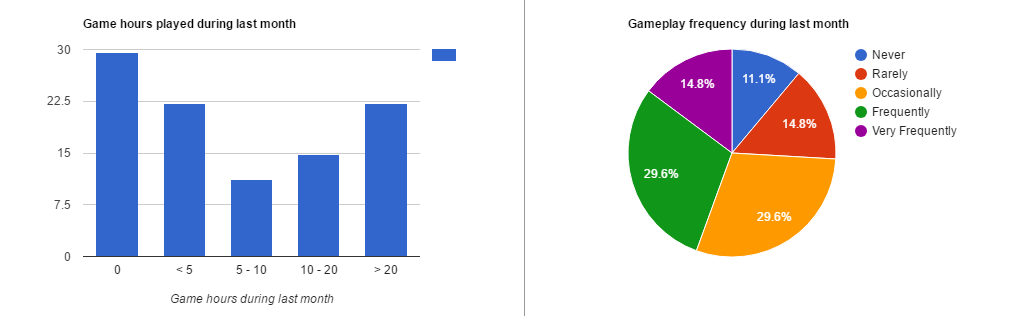
\includegraphics[width=\linewidth]{figures/experiment2/game-prequestionnaire.PNG}
    \caption{Results on participants' gameplay frequency for Experiment 2}
    \label{fig:game-prequestionnaire}
\end{figure}

\subsection{Annotation Performance}
%DBPedia autmatoc likinng accuracy - 228
All the data used in the game has been automatically generated by the framework. The only task which was manually performed by the experimenter was uploading the MSNBC documents into the framework through the admin interface. The rest was carried out automatically from recognizing the entities to generating the corresponding Dbpedia candidates. 

Regardig the number of entities available in the MSNBC dataset, our NER microservice recognized 228 entity mentions in total. Corresponding F-Measures were used to calculate the performance of the entity recognition service using MSNBC dataset and resulted with 0.77 for precision, 0.83 for recall and 0.8 for the f-score. The performance of other automatic annotators in terms of entity recognition are presented in Table \ref{tab:ex2-ner-performance}. We observe a very small improvement on the overall F-score of our framework compared to AIDA which performed best among the other automatic annotator. However, improving entity recognition performance is not the scope of this study and therefore we will not elaborate on the respective \ac{ner} performance results. 

% Table generated by Excel2LaTeX from sheet 'Sheet4'
\begin{table}[htbp]
  \centering
  \caption{NER performance on MSNBC dataset}
    \begin{tabular}{|l|c|c|c|}
    \toprule
    \textbf{-/Dataset} & \multicolumn{3}{c|}{\textbf{MSNBC Dataset}} \\
    \midrule
    \textbf{Annotator/Metric} & \multicolumn{1}{l|}{\textbf{Precision}} & \multicolumn{1}{l|}{\textbf{Recall}} & \multicolumn{1}{l|}{\textbf{F-Score}} \\
    \midrule
    \textbf{Babelfy} & 0.45  & 0.65  & 0.52 \\
    \midrule
    \textbf{Dbpedia Spotlight} & 0.58  & 0.6   & 0.57 \\
    \midrule
    \textbf{AIDA} & 0.92  & 0.71  & 0.78 \\
    \midrule
    \textbf{Dexter} & 0.49  & 0.66  & 0.39 \\
    \midrule
    \textbf{Fastype (Experiment 2)} & \textcolor[rgb]{ 1,  0,  0}{\textbf{0.77}} & \textcolor[rgb]{ 1,  0,  0}{\textbf{0.83}} & \textcolor[rgb]{ 1,  0,  0}{\textbf{0.8}} \\
    \bottomrule
    \end{tabular}%
  \label{tab:ex2-ner-performance}%
\end{table}%

%24 entities 
The performance of the automatic annotator used by our framework, namely Dbpedia Spotlight, in terms of accuracy of linking the identified entities with the correct candidate has been calculated as well. When querying Spotlight for a specific entity, a list of candidates is returned correspondingly with each candidate associated with a final score. The candidate with the highest final score is considered by Spotlight to be the correct link associated with the target entity. We run our analysis on all the 228 recognized entities and checked for each entity whether the associated candidate with the highest final score was the correct representative based on the gold standard of MSNBC provided by GERBIL \cite{40}. Among the 228 recognized entities, Spotlight linked 66.35\% of them correctly and 33.65\% incorrectly. This shows a significant improvement compared to the datasets used in the first experiment. A possible explanation for the observed improvement is the nature of the dataset. The entities recognized in MSNBC have a less ambiguous nature compared to the KORE50 and Spotlight datasets used in the first experiment. As a result the automatic annotator improved its performance. 

Before proceeding with reporting on the performances of the non-expert annotators, we report on the total number of entities resolved during the experiment. The assessment technique used for evaluating an entity based on the participants judgment is the same as for the first. The game accumulates four different judgments from independent annotators before resolving an entity with a specific candidate. Among the 228 entities recognized in total, only 24 of them were resolved while the second experiment was being conducted. Unfortunately, this is 60\% less entities resolved in the second experiment compared to the first experiment. The reason for this outome is because the average tasks/game-rounds completed during a session dropped significantly for the game. The game elements such as fast typing, bonus questions, bets and challenges are all additional tasks that take significant amount of time to complete. Besides the fact that the game elements enrich the experience, improve player engagement and increase intrinsic motivation, they did slow down the annotation process significantly more compared to AnnotateMe Interface. One might argue that drawing conclusions on such a small sample of resolved entities does not necessarily generalize to the whole population. We recognize this issue in our analysis and therefore we address it as a limitation on our results. However, the potential of the game is significantly higher compared to the plain interface used in the first experiment and we predict that the game will still perform much better in terms of user engagement and maintain annotation quality regardless of the number of annotations resolved. 

%ANOVA difference between DBpedia anntator and human - in accuracy (report the f-scores)
Among the 26 resolved entities 95\% were correctly linked with a Dbpedia candidate whereas 5\% were incorrectly linked when compared to the gold standard. Table \ref{tab:ex2-annotation-performance} shows the performance of the game and Dbpedia Spotlight on all 26 resolved entities in terms of precision, recall and f-score measures. The game which used non-expert annotators exhibits a slight improvement compared to the automatic annotator. However, after running a one-way Anova, the differences between the two groups are not statistically significant for p = 0.05. Regardless, for the entities that have been resolved, the annotation quality remained unchanged as compared to the first experiment, with a very small improvement for the second experiment. With the results acquired so far, the third hypothesis (H2.3) for the second experiment is supported. 

% Table generated by Excel2LaTeX from sheet 'Sheet5'
\begin{table}[htbp]
  \centering
  \caption{Annotation Performance - Experiment 2}
    \begin{tabular}{|l|r|r|r|l|}
    \toprule
    \multicolumn{5}{|c|}{\textbf{Precision, Recall, F-Scores}} \\
    \midrule
    \textbf{Annotator} & \multicolumn{1}{l|}{\textbf{Precision}} & \multicolumn{1}{l|}{\textbf{Recall}} & \multicolumn{1}{l|}{\textbf{F-Score}} & \textbf{DATASET} \\
    \midrule
    \rowcolor \textcolor[rgb]{ .8,  0,  0}{\textbf{Game}} & \textcolor[rgb]{ .8,  0,  0}{\textbf{0.87}} & \textcolor[rgb]{ .8,  0,  0}{\textbf{0.95}} & \textcolor[rgb]{ .8,  0,  0}{\textbf{0.91}} & \textcolor[rgb]{ .8,  0,  0}{\textbf{MSNBC Dataset}} \\
    \midrule
    Dbpedia Spotlight & 0.85  & 0.81  & 0.8   & MSNBC Dataset \\
    \bottomrule
    \end{tabular}%
  \label{tab:ex2-annotation-performance}%
\end{table}%


%agreement level  - ANOVA differences
In the first experiment we reported on the agreement levels of participants which represents the ratio of correct answers given compared to the total number of answers. Even though the annotation quality remained the same, the agreement level experienced a significant drop during the second experiment. Figure \ref{fig:game-agreement-level} presents the agreement levels of all participants for the second experiment. The average agreement level for an individual participants for the second experiment is 32\% which is significantly less than compared with the first experiment which was 51\%. Please note that the agreement levels do not take into consideration annotation data for entities that have not yet been resolved. For example if three participants have selected the same candidate for a specific entity, this means that they agree on that specific candidate. However, unless a fourth participant selects the same candidate, the entity is not resolved and therefore the other three participants are not credited for having agreed with each other. We argue that the performance drop is a result of having 60\% less data for the second experiment to analyze and provide results as compared to the first experiment. 

\begin{figure}[]
    \centering
    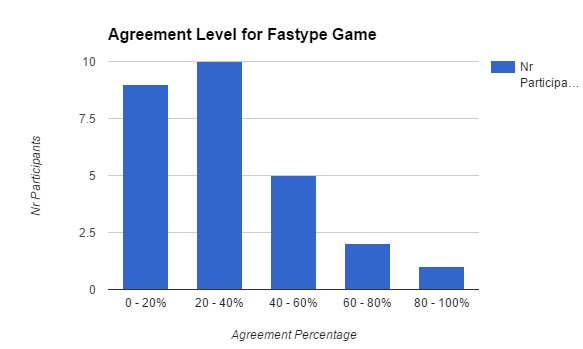
\includegraphics[width=\linewidth]{figures/experiment2/ex2-agreementlevel.PNG}
    \caption{Participant's Agreement Level for Experiment 2}
    \label{fig:game-agreement-level}
\end{figure}

\subsection{Game Design Analysis}
In the previous sub-sections we reported on the performances of non-expert human annotators in terms of annotation quality and agreement level and saw that the quality of annotations did not experience any decrease. In this subsection we report on the performance of Fastype in terms of playfulness, player engagement and see if the players were intrinsically motivated to participate and play the game. 

One of the metrics used to assess the playfulness or the attractiveness of both interfaces (AnnotateMe and Fastype) was by measuring the number of the so-called \textit{free-will annotations}. When conducting each experiment, the participants were instructed to perform their tasks continuously until instructed to stop. An annotation was considered to be a \textit{free-will annotation} when participants free-willingly decided to continue performing tasks even after the experimenter informed them that they have already completed the number of obligatory annotations and were allowed to finish the experiment. Table \ref{tab:free-will-annotation-res} shows the results of free-will annotations performed in both experiments in addition to the average number of tasks performed in a session. The game exhibits a slight improvement over the plain interface in terms of free-will annotations, however, the calculation of one-way Anova resulted in statistically insignificant difference for p = 0.05. The reason for the insignificant difference can be explained by observing the second row of the table, namely, the average annotations performed during an experiment session. We observe that participants performed 50\% more annotations using the plain interface as opposed to the game. Besides the fact that the difference was not significant, we argue that an average of 23\% free-will annotations over an average of 10 game rounds performed by a single participants is better than an average of 17\% free-will annotations over an average of 22 annotation rounds. In a long run, we are confident that the game would perform significantly better and have a significant higher attractiveness as compared to the plain interface. The results presented in Figure \ref{fig:participants-perference} easily back up this claim. 

% Table generated by Excel2LaTeX from sheet 'Sheet6'
\begin{table}[htbp]
  \centering
  \caption{Results of free-will annotations for experiment 1 and 2}
    \begin{tabular}{|l|r|r|}
    \toprule
    \multicolumn{3}{|c|}{\textbf{Participant Average Freewill and total annotations performed}} \\
    \midrule
          & \multicolumn{1}{l|}{\textbf{Fastype Game}} & \multicolumn{1}{l|}{\textbf{AnnotateMe Interface}} \\
    \midrule
    \textbf{Average of free-will annotations} & 23\%    & 17\% \\
    \midrule
    \textbf{Average annotations performed} & 10    & 22 \\
    \bottomrule
    \end{tabular}%
  \label{tab:free-will-annotation-res}%
\end{table}%


\begin{figure}[]
    \centering
    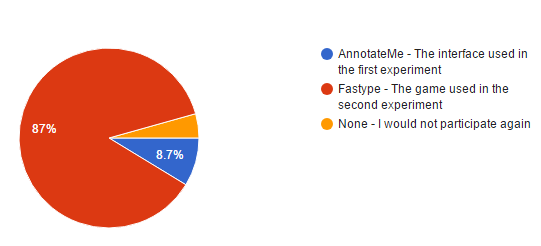
\includegraphics[width=\linewidth]{figures/experiment2/participant-preferance.PNG}
    \caption{Participant's preferred interface for performing annotations}
    \label{fig:participants-perference}
\end{figure}

After both experiments were conducted, we asked participants that took part in both experiments to fill-in a final questionnaire regarding their preferred interface in case they would be asked to do a third experiment. As seen from Figure \ref{fig:participants-perference}, the majority of participants preferred the game compared to AnnotateMe Interface. Please note that the participants had the possibility to choose a third option which allowed participants to express feelings of neutrality or dislike for both interfaces. The third option was provided as a measure against potential bias in our results by allowing all participants who disliked both experience to freely express it. The questionnaire was completely anonymous and was sent through emails where participants completed it from home.

%Post Questionnaire
A post-questionnaire assessing the overall design of the game was also used in the second experiment. In the post-questionnaire, participants were asked different type of questions with each contributing to the assessment of different aspects of game design. Additionally, in order to compare the attractiveness and engagement of participants with the game and the plain interface, both designs were assessed using similar questions in both post-questionnaires. 

%Anova analysis towards experience with interfaces
In order to assess the attractiveness of each interface we asked participants to rate their experience with each interface. The results of the first experiment are shown in the top-right graph presented in Figure \ref{fig:ex1-postresults} whereas the results of the second experiment are presented in Figure \ref{fig:game-experience}. To make sure that the game was perceived as significantly more attractive and fun to use as compared to the plain interface, we run one-way Anova analysis and the results confirm that the difference is statistically significant for p = 0.05 and for p = 0.01. This indicates that the game was perceived significantly more attractive as opposed to the plain interface.

\begin{figure}[]
    \centering
    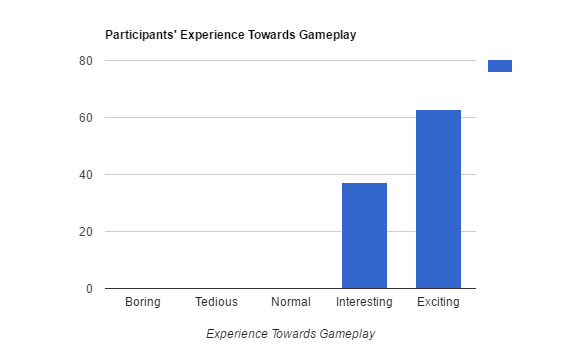
\includegraphics[width=\linewidth]{figures/experiment2/game-participant-experience.PNG}
    \caption{Participant's experience towards the gameplay}
    \label{fig:game-experience}
\end{figure}

%anova analysis about egagement frequency
Regarding the user's perceived engagement with both interfaces, we asked participants how often they would use each interface outside the experiment. Please note that for the same question we unfortunately used different type of answers, with the answer for the first experiment being labels ranging from "Definitely Not" to "Definitely", and the answer for the second experiment being a 7-point liker scale ranging from "Never Again" to "A Lot". However, when calculating one-way Anova, we normalized the 7-point liker scale to 5-point liker scale (dividing the value with 7 and than multiplying it with 5) to be able to properly compare the two observations together (See Appendix \ref{appendix3:engagement_analysis}). The results of the one-way Anova report a statistically significant difference between the two observation for p = 0.05 as well as p = 0.05. These results indicate that the game was perceived as significantly more engaging than the plain interface.  


\begin{figure}[]
    \centering
    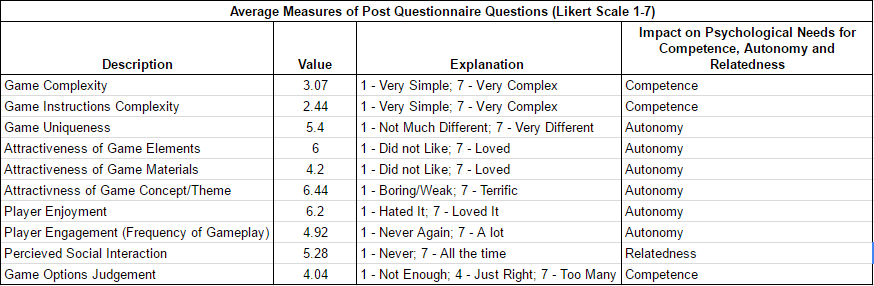
\includegraphics[width=\linewidth]{figures/experiment2/post-questionnaire-final.PNG}
    \caption{Results from the post-questionnaire analysis for experiment 2}
    \label{fig:post-questionnaire-final}
\end{figure}

Finally, Figure \ref{fig:post-questionnaire-final} presents a table with the final results for the rest of the questions used to assess the design of the game on the post-questionnaire. It can be observed that the game scores relatively well in all of the design questions presented to the participants. The table also illustrates the impact of the different game design elements on basic psychological needs for autonomy, competence and relatedness which represent the main factors for affecting player's intrinsic motivation. Since the players perceived the game as generally enjoyable, engaging, socially intractable, easy to adapt with the instruction and rules of the game, genuinely liked the elements, materials and the theme of the game, we claim that the participants were intrinsically motivated to play and do not rely in any other incentive but the desire to be entertained. Consequently, based on these acquired results the first hypothesis of the second experiment is supported (H2.1). The second hypothesis (H2.2) is also supported since the one-way Anova analysis indicate that the participants preferred to use the game significantly more than using the plain interface.  